

%--------------------------------------------------
\section{Modelo de entidades del negocio}

\begin{figure}[htbp!]
	\centering
		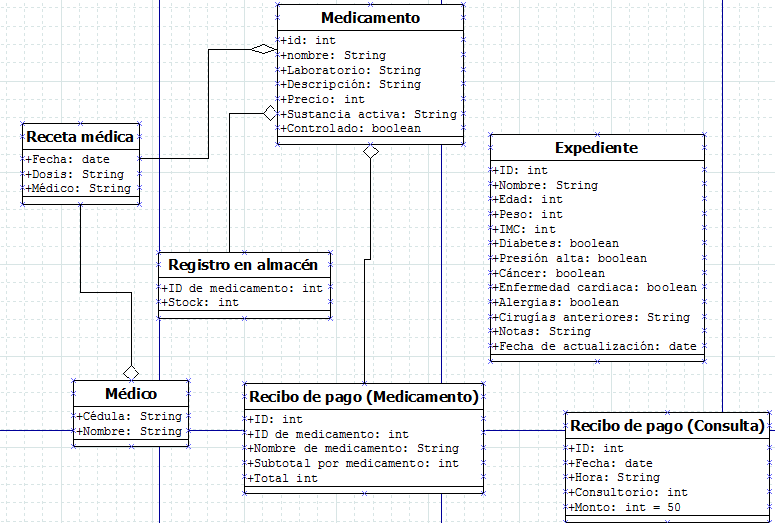
\includegraphics[width=1\textwidth]{images/entidades}
		\caption{Modelo de entidades del negocio.}
	\end{figure}


%--------------------------------------------------
\section{Descripción de atributos}
A continuaci\'on se describen cada uno de los atributos de las entidades mostradas en el diagrama anterior.

% - - - - - - - - - - - - - - - - - - - - - - - - -
\subsection{Atributos de ``Medicamento''}

\begin{description}
	\item[ID: ] Permite identificar a cada uno de los medicamentos. Es \'unico por medicamento.
	\item[Nombre: ] Nombre del medicamento.
	\item[Laboratorio: ] Nombre del laboratorio que produce tal medicamento.
	\item[Descripci\'on: ] Res\'umen que describe la forma en la que el medicamento est\'a, cu\'antas unidades contiene un recipiente del mismo, y el peso o vol\'umen de cada unidad.
	\item[Precio: ] Precio que cuesta el recipiente con $X$ unidades de medicamento, descrito en el atributo "`Descripci\'on"'.
	\item[Sustancia Activa: ] Indica la o las sustancias activas que componen el medicamento. 
	\item[Controlado: ] Es una bandera que indica si el medicamento es controlado o no.
\end{description}
% - - - - - - - - - - - - - - - - - - - - - - - - -
\subsection{Atributos de ``Expediente''}

\begin{description}
	\item[ID: ] Identificador del expediente. Es \'unico por cada uno.
	\item[Nombre: ] Nombre del paciente al que pertenece el expediente.
	\item[Edad: ] Edad del paciente.
	\item[Peso: ] Peso del paciente.
	\item[IMC: ] \'Indice de masa corporal del paciente.
	\item[Diabetes: ] Bandera que indica si el paciente sufre de diabetes.
	\item[Presi\'on alta: ] Bandera que indica si el paciente sufre de presi\'on alta.
	\item[C\'ancer: ] Bandera que indica si el paciente sufre de alg\'un tipo de c\'ancer.
	\item[Enfermedad cardiaca: ] Bandera que indica si el paciente sufre de alguna enfermedad cardiaca.
	\item[Alergias: ] Describe las alergias que el paciente tiene, en caso de tenerlas.
	\item[Cirug\'ias anteriores: ] Indica las cirugias que el paciente ha recibido, en caso de tener. 
	\item[Notas: ] Indican cualquier observaci\'on que el m\'edico haya tenido sobre el paciente.
	\item[Fecha de actualizaci\'on: ] Fecha en la que se realiz\'o la \'ultima actualizaci\'on al expediente.
\end{description}

% - - - - - - - - - - - - - - - - - - - - - - - - -
\subsection{Atributos de ``Registro en almac\'en''}

\begin{description}
	\item[ID de medicamento: ] Identificador del medicamento sobre el cual hace referencia el stock.
	\item[Stock: ] Cantidad de unidades que se tienen el medicamento con ID $[ID de medicamento]$.
\end{description}
% - - - - - - - - - - - - - - - - - - - - - - - - -
\subsection{Atributos de ``Receta m\'edica''}

\begin{description}
	\item[Fecha: ] Indica la fecha en la que la receta fue expedida.
	\item[ID de medicamento: ] Identificador del medicamento con el cual est\'a registrado en el sistema.
	\item[Nombre de medicamento: ] Nombre del medicamento al cual el ID de medicamento al cual hace referencia.
	\item[Dosis: ] Cantidad que el paciente debe ingerir del medicamento en un periodo definido.
	\item[M\'edico: ] Nombre del m\'edico que gener\'o la receta.
\end{description}
% - - - - - - - - - - - - - - - - - - - - - - - - -
\subsection{Atributos de ``Recibo de pago (Consulta)''}

\begin{description}
	\item[ID: ] Identifica el n\'umero de transacci\'on, con el cual la cita podr\'a ser pagada en caja.
	\item[Fecha: ] Fecha en la cual la consulta m\'edica ser\'ia realizada.
	\item[Hora: ] Hora en la cual la consulta m\'edica ser\'ia realizada.
	\item[Consultorio: ] N\'umero que indica el consultorio en el cual la consulta m\'edica ser\'ia realizada.
	\item[Monto: ] Indica la cantidad que debe ser pagada en caja, correspondiente a la cita. Para el proceso actual, el monto es siempre de \$ 50 MXN.
	\item[M\'edico: ] Nombre del m\'edico que gener\'o la receta.
\end{description}
% - - - - - - - - - - - - - - - - - - - - - - - - -
\subsection{Atributos de ``Recibo de pago (Medicamentos)''}

\begin{description}
	\item[ID: ] Identifica el n\'umero de transacci\'on, con el cual la cita podr\'a ser pagada en caja.
	\item[*ID de medicamento: ] Identificador del medicamento con el cual est\'a registrado en el sistema.
	\item[*Nombre de medicamento: ] Nombre del medicamento al cual el ID de medicamento al cual hace referencia.
	\item[*Subtotal por medicamento: ] Indica la cantidad a pagar por cada medicamento. Si hay varios medicamentos de un mismo tipo el subtotal es igual a la suma de los subtotales individules.
	\item[Total: ] Indica el costo total de los medicamentos. El costo total es igual a la suma de los subtotales.
	
	NOTA: '*' indica que el atributo puede repetirse varias veces en un mismo recibo de pago.
\end{description}
% - - - - - - - - - - - - - - - - - - - - - - - - -


